\documentclass[11pt]{article}

\usepackage[a4paper,margin=1in]{geometry}
\usepackage[T1]{fontenc}
\usepackage[utf8]{inputenc}
\usepackage{lmodern}
\usepackage{microtype}
\usepackage{amsmath,amssymb,amsthm,mathtools}
\usepackage{booktabs}
\usepackage{graphicx}
\usepackage{enumitem}
\usepackage[numbers,sort&compress]{natbib}
\usepackage{xcolor}
\usepackage{xurl}
\usepackage[colorlinks=true,linkcolor=blue!55!black,citecolor=blue!55!black,urlcolor=blue!55!black]{hyperref}
\usepackage[nameinlink,noabbrev]{cleveref}

\setlength{\parindent}{1.4em}
\setlength{\parskip}{0.15em}
\setlist{itemsep=0.25em,topsep=0.35em}

\newtheorem{theorem}{Theorem}[section]
\newtheorem{proposition}[theorem]{Proposition}
\newtheorem{lemma}[theorem]{Lemma}
\newtheorem{corollary}[theorem]{Corollary}
\theoremstyle{definition}
\newtheorem{definition}[theorem]{Definition}
\theoremstyle{remark}
\newtheorem{remark}[theorem]{Remark}

\newcommand{\R}{\mathbb R}
\newcommand{\C}{\mathbb C}
\newcommand{\cK}{\mathcal K}
\newcommand{\cA}{\mathcal A}
\newcommand{\cQ}{\mathcal Q}
\newcommand{\cB}{\mathcal B}
\newcommand{\cC}{\mathcal C}
\newcommand{\cE}{\mathcal E}
\newcommand{\uc}{u_{\mathrm c}}
\newcommand{\Id}{\operatorname{Id}}
\newcommand{\spec}{\operatorname{spec}}
\newcommand{\tr}{\operatorname{tr}}
\newcommand{\Span}{\operatorname{span}}
\newcommand{\norm}[1]{\left\lVert #1\right\rVert}
\newcommand{\one}{\mathbf 1}

\title{\textbf{Time-Ordered Cycle Curvature for Gaussian}\
\textbf{Quadratic Markov Cocycles}\\
\large Two-Step Spectral Blindness, Commutator Response, and\\[-0.1em]
\large Parity-Compatible Directed Traces}
\author{Liang Wang\\
\small School of Artificial Intelligence and Automation,\\[-0.2em]
\small Huazhong University of Science and Technology, Wuhan 430074, P.R. China\\
\small \texttt{wangliang.f@gmail.com}}
\date{July 2026}

\begin{document}

\maketitle

\begin{abstract}
Frozen cycle traces encode the resonances of a Gaussian quadratic Markov
operator, but they do not determine which scalar spectral quantities retain
the order of a non-autonomous drive.  We identify an exact obstruction and
construct the first nontrivial time-directed replacements.

Let $\cK_u$ be the normalized fixed-noise kernel centered at
$f_u(x)=1-u x^2$ on $[-1,1]$.  Each $\cK_u$ is Hilbert--Schmidt, so every
two-step block $\cK_a\cK_b$ is trace class.  Nevertheless,
\[
 \spec(\cK_a\cK_b)\setminus\{0\}
 =\spec(\cK_b\cK_a)\setminus\{0\},
 \qquad
 \det(I-z\cK_a\cK_b)=\det(I-z\cK_b\cK_a).
\]
Thus no two-step eigenvalue or Fredholm determinant can detect reversal inside
one pair.  Order is not absent: for symmetric parameters,
\[
 \cK_{u-\varepsilon}\cK_{u+\varepsilon}
 -\cK_{u+\varepsilon}\cK_{u-\varepsilon}
 =2\varepsilon[\cK_u,\cK_u']+O(\varepsilon^3).
\]
The stationary measures and every separating state--observable expectation
have corresponding first-order responses, although the spectra remain
identical.

For the logarithmic schedule
$u_n=\uc+\kappa(\log(n+c))^{-p}$, paired commutator corrections are summable
but have a nonzero renormalized tail.  If $m_j=(u_{2j-1}+u_{2j})/2$, then in
operator norm
\[
 (\log(2J+c))^p\sum_{j\ge J}
 \left(\cK_{u_{2j-1}}\cK_{u_{2j}}-\cK_{m_j}^2\right)
 \longrightarrow-\frac{\kappa}{4}[\cK_{\uc},\cK_{\uc}'].
\]

The minimal scalar orientation trace requires three parameter values:
\[
 \Omega_{\cA}(a,b,c)
 =\tr\bigl(\cA_a[\cA_b,\cA_c]\bigr).
\]
For every analytic Hilbert--Schmidt family it factors exactly as
\[
 \Omega_{\cA}(a,b,c)
 =(a-b)(b-c)(c-a)G_{\cA}(a,b,c),
 \quad
 G_{\cA}(u,u,u)=\frac12\tr\bigl(\cA_u[\cA_u',\cA_u'']\bigr).
\]
Taking $\cA_u=\cK_u^2$ gives the minimal parity-compatible scalar, a directed
six-step trace.  Under a macroscopic logarithmic schedule its first nonzero
scale is $(\log T)^{-3p-3}$; consecutive directed traces are of order
$n^{-3}(\log n)^{-3p-3}$ and are absolutely summable.

Target-independent computations verify two-step spectral coincidence to
$5.3\times10^{-12}$ while the matrices, stationary laws, and observables
differ linearly in $\varepsilon$.  The one-step and parity-block orientation
curvatures are nonzero and converge under midpoint discretization at order
$d^{-2}$.  The results close the route through raw two-step eigenphases but
leave a precise commutator and directed-determinant route.  No Riemann zero or
arithmetic target is used.
\end{abstract}

\noindent\textbf{Keywords:} non-autonomous Markov operator; time ordering;
commutator; Fredholm determinant; orientation curvature; parity block;
logarithmic schedule.

\medskip
\noindent\textbf{MSC 2020:} 47A10; 47B47; 47G10; 37H20; 60J10; 65R20.

\section{Introduction}

A non-autonomous product remembers order at the operator level, but not every
spectral statistic does.  The elementary identity that $AB$ and $BA$ have the
same nonzero spectrum becomes a serious obstruction when a two-step block is
proposed as the primitive time-directed observable.  Eigenvectors, invariant
measures, and subsequent products can change under reversal even while all
nonzero eigenvalues and the complete Fredholm determinant remain fixed.

This distinction is relevant near the first quadratic band-merging parameter
\begin{equation}\label{eq:uc}
 \uc^3-2\uc^2+2\uc-2=0,
 \qquad \uc=1.543689012692\ldots.
\end{equation}
The deterministic map has a period-two decomposition and a parity eigenvalue
$-1$, so the natural autonomous primitive is a two-step block
\citep{WangParity2026}.  Gaussian smoothing turns the finite matrices into a
compact analytic continuum Markov family, and midpoint matrices recover its
nonzero isolated resonances \citep{WangGaussianResponse2026,WangContinuum2026}.
The preceding paper then constructed centered cycle traces and a regularized
determinant for each frozen operator \citep{WangCycleSpectrum2026}.

The remaining issue is temporal.  An unweighted operator average forgets
order, and its first logarithmic response depends only on the mean parameter
offset \citep{WangObstructions2026}.  Products are order sensitive, often
organized through commutator or Magnus-type expansions
\citep{BlanesEtAl2009}, but a claim about a product spectrum must still specify
which order information survives cyclic trace invariance.

The present paper supplies that audit.  The first result is negative and
exact: one paired spectrum is blind to reversal.  The positive replacement
has two levels.  At operator level, a first-order commutator changes
stationary laws and observable responses.  At scalar level, the minimal
directed trace needs three factors and begins cubically in parameter
separations.  If parity blocks are retained, the minimal scalar uses three
two-step blocks, hence six one-step kernels.

The logarithmic schedule separates these levels sharply.  Accumulated
within-pair commutators survive at the same $(\log J)^{-p}$ tail scale as the
ordinary response.  A scalar orientation trace at three macroscopic times is
smaller, of order $(\log T)^{-3p-3}$, while the consecutive version is
summable.  This scale hierarchy determines what a future cocycle or trace
formula can plausibly measure.

\subsection*{Main results}

\begin{enumerate}[label=\textbf{R\arabic*.},leftmargin=3.2em]
 \item Every two-step product $\cK_a\cK_b$ is trace class, but reversal
 preserves its entire nonzero spectrum and Fredholm determinant.  The two
 stationary measures are transported into one another by one factor.

 \item Symmetric order reversal has the operator expansion
 $2\varepsilon[\cK,\cK']+O(\varepsilon^3)$.  A Poisson equation gives the
 first stationary response, so order remains visible to states and
 observables despite spectral blindness.

 \item For a logarithmic drive, the sum of late paired corrections converges
 in operator norm and has the explicit renormalized commutator limit
 $-(\kappa/4)[\cK_{\uc},\cK_{\uc}']$.

 \item The three-factor directed trace is a fully alternating analytic
 function of its parameters.  It factors by the Vandermonde polynomial, and
 its diagonal quotient is the intrinsic orientation curvature
 $\frac12\tr(\cA[\cA',\cA''])$.

 \item The frozen parity family $\cQ_u=\cK_u^2$ yields a directed six-step
 trace.  This is the minimal parity-compatible scalar that distinguishes an
 ordering of frozen blocks.

 \item Macroscopic and consecutive logarithmic schedules have exact directed
 scales.  Midpoint approximations of both curvatures converge as $d^{-2}$,
 and all predicted small-separation powers are recovered numerically.
\end{enumerate}

\subsection*{Scope}

The paper studies fixed $\sigma>0$.  It proves statements about Markov
products, trace ideals, and logarithmic schedules, not a small-noise theorem.
The numerical widths are untuned, no Riemann zero is loaded, and no Markov
product is identified with a self-adjoint energy operator.  In particular,
the paper tests one proposed bridge in a longer Hilbert--P\'olya research
program; it does not assert that another bridge exists
\citep{BerryKeating1999}.

\section{Fixed-noise operators and two-step trace ideals}
\label{sec:operators}

Let $I=[-1,1]$, fix $\sigma>0$, and put
\begin{align}
 f_u(x)&=1-u x^2,\label{eq:map}\\
 w_u(x,y)&=\exp\left[-\frac{(y-f_u(x))^2}{2\sigma^2}\right],\\
 Z_u(x)&=\int_Iw_u(x,z)\,dz,
 \qquad q_u(x,y)=\frac{w_u(x,y)}{Z_u(x)}.\label{eq:kernel}
\end{align}
The observable Markov operator is
\begin{equation}\label{eq:operator}
 (\cK_u g)(x)=\int_Iq_u(x,y)g(y)\,dy.
\end{equation}
On $C(I)$ it is a compact strongly positive contraction with
$\cK_u\one=\one$.  On $H=L^2(I,dx)$ it is Hilbert--Schmidt.  The family is
analytic in operator norm on $C(I)$ and in Hilbert--Schmidt norm on $H$; all
kernel derivatives are smooth and bounded on compact parameter intervals
\citep{Kress2014,WangContinuum2026}.

Write $\mathfrak S_1(H)$ and $\mathfrak S_2(H)$ for the trace-class and
Hilbert--Schmidt ideals.  Since the product of two Hilbert--Schmidt operators
is trace class,
\begin{equation}\label{eq:block}
 \cB_{a,b}=\cK_a\cK_b\in\mathfrak S_1(H).
\end{equation}
It remains a strongly positive Markov operator on $C(I)$; hence its Perron
root $1$ is algebraically simple.

\section{Two-step spectral blindness}
\label{sec:blindness}

\begin{theorem}[Reversal-invariant two-step spectrum]
\label{thm:ab-ba}
For every real $a,b$,
\begin{equation}\label{eq:ab-spectrum}
 \spec(\cB_{a,b})\setminus\{0\}
 =\spec(\cB_{b,a})\setminus\{0\},
\end{equation}
including algebraic multiplicity and Jordan structure.  Moreover, for every
$z\in\C$,
\begin{equation}\label{eq:sylvester}
 \det(I-z\cK_a\cK_b)=\det(I-z\cK_b\cK_a).
\end{equation}
After removing the simple Perron factor, the entire non-Perron determinants
\begin{equation}\label{eq:two-step-centered-det}
 \Delta_{a,b}(z)=\frac{\det(I-z\cK_a\cK_b)}{1-z}
\end{equation}
satisfy $\Delta_{a,b}=\Delta_{b,a}$.
\end{theorem}

\begin{proof}
For bounded operators $A,B$, the maps $B$ and $A$ identify the generalized
eigenspaces of $AB$ and $BA$ at every $\lambda\ne0$.  This gives
\eqref{eq:ab-spectrum}.  Because $\cK_a,\cK_b\in\mathfrak S_2$, both products
are trace class.  The trace-ideal Sylvester identity gives
\eqref{eq:sylvester} \citep{GohbergEtAl2000,Simon2005}.  Strong positivity
makes the zero of the determinant at $z=1$ simple, so division gives the
entire identity for $\Delta$.
\end{proof}

The spectrum is blind, but the eigenvectors are not.  If
$\cK_a\cK_b r=\lambda r$ with $\lambda\ne0$, then $\cK_b r$ is a generalized
eigenvector of $\cK_b\cK_a$ at the same eigenvalue.  This transport depends on
the order.

\begin{proposition}[Exact stationary transport]
\label{prop:stationary-transport}
Let $\pi_{a,b}$ be the unique invariant probability of $\cK_a\cK_b$.  Then
\begin{equation}\label{eq:stationary-transport}
 \pi_{b,a}=\pi_{a,b}\cK_a,
 \qquad
 \pi_{a,b}=\pi_{b,a}\cK_b.
\end{equation}
\end{proposition}

\begin{proof}
Since $\cK_a\one=\one$, $\pi_{a,b}\cK_a$ is a probability.  Associativity and
invariance give
\[
 (\pi_{a,b}\cK_a)(\cK_b\cK_a)
 =\pi_{a,b}(\cK_a\cK_b)\cK_a
 =\pi_{a,b}\cK_a.
\]
Uniqueness of the invariant probability proves the first identity.  The
second is symmetric.
\end{proof}

Thus equality of eigenvalues cannot be promoted to equality of the two
Markov dynamics.  A statistic based only on the eigenvalues of one two-step
block cannot identify which kernel came first.

\section{Commutator response inside one pair}
\label{sec:commutator}

Fix $u$ and abbreviate
\[
 \cK=\cK_u,
 \qquad \dot\cK=\partial_u\cK_u,
 \qquad \ddot\cK=\partial_u^2\cK_u,
 \qquad \cC_u=[\cK_u,\cK_u'].
\]
Define the forward and reversed symmetric blocks
\begin{equation}\label{eq:arrows}
 \cB_\to(u,\varepsilon)
 =\cK_{u-\varepsilon}\cK_{u+\varepsilon},
 \qquad
 \cB_\leftarrow(u,\varepsilon)
 =\cK_{u+\varepsilon}\cK_{u-\varepsilon}.
\end{equation}

\begin{theorem}[Two-step commutator expansion]
\label{thm:commutator}
Locally uniformly in $u$, in operator norm on $C(I)$ and trace norm on $H$,
\begin{align}
 \cB_\to(u,\varepsilon)
 &=\cK^2+\varepsilon[\cK,\dot\cK]
 +\varepsilon^2\left\{
 \frac12(\cK\ddot\cK+\ddot\cK\cK)-\dot\cK^2
 \right\}+O(\varepsilon^3),\label{eq:forward-expansion}\\
 \cB_\to(u,\varepsilon)-\cB_\leftarrow(u,\varepsilon)
 &=2\varepsilon[\cK,\dot\cK]+O(\varepsilon^3).
 \label{eq:commutator-expansion}
\end{align}
In particular, the leading order difference is traceless and invisible to
the determinant in \cref{thm:ab-ba}.
\end{theorem}

\begin{proof}
Insert the operator-norm Taylor expansions
\[
 \cK_{u\pm\varepsilon}
 =\cK\pm\varepsilon\dot\cK
 +\frac{\varepsilon^2}{2}\ddot\cK+O(\varepsilon^3)
\]
and multiply.  Reversal is equivalent to replacing $\varepsilon$ by
$-\varepsilon$, so all even terms cancel in the difference.  The products of
two Hilbert--Schmidt remainders give the same expansion in trace norm.
\end{proof}

The first-order change can be seen by a state and an observable:
\begin{equation}\label{eq:weak-order-response}
 \mu\left(\cB_\to-\cB_\leftarrow\right)g
 =2\varepsilon\,\mu[\cK,\dot\cK]g+O_{\mu,g}(\varepsilon^3).
\end{equation}
It also changes the stationary law.  Let $\pi_u$ be invariant for $\cK_u$.

\begin{proposition}[Stationary order response]
\label{prop:stationary-response}
There is a unique signed measure $\eta_u$ satisfying
\begin{equation}\label{eq:poisson}
 \eta_u(I-\cK_u^2)=\pi_u[\cK_u,\cK_u'],
 \qquad \eta_u(\one)=0.
\end{equation}
In total variation,
\begin{equation}\label{eq:stationary-expansion}
 \pi_\to(u,\varepsilon)-\pi_\leftarrow(u,\varepsilon)
 =2\varepsilon\eta_u+O(\varepsilon^3).
\end{equation}
\end{proposition}

\begin{proof}
The fixed-noise kernel has a simple Perron root and all other spectral values
strictly inside the unit disk.  Thus $I-(\cK_u^*)^2$ is invertible on the
zero-mass measures \citep{Seneta2006,WangCycleSpectrum2026}, proving existence
and uniqueness in \eqref{eq:poisson}.  Differentiate the stationarity equation
for \eqref{eq:forward-expansion}; its first derivative is exactly
\eqref{eq:poisson}.  Since reversal sends $\varepsilon$ to $-\varepsilon$, the
stationary difference is odd and the next term is cubic
\citep{Kato1995}.
\end{proof}

\subsection{Renormalized tail of a logarithmic pairing}

Let
\begin{equation}\label{eq:schedule}
 u_n=\uc+\frac{\kappa}{(\log(n+c))^p},
 \qquad c>1,\quad p>0.
\end{equation}
For pair $j$, put
\begin{equation}\label{eq:pair-coordinates}
 m_j=\frac{u_{2j-1}+u_{2j}}2,
 \qquad
 \varepsilon_j=\frac{u_{2j}-u_{2j-1}}2,
 \qquad
 L_J=\log(2J+c).
\end{equation}

\begin{theorem}[Summable pair order and its renormalized tail]
\label{thm:pair-tail}
The series
\begin{equation}\label{eq:tail-operator}
 \cE_J=\sum_{j=J}^{\infty}
 \left(\cK_{u_{2j-1}}\cK_{u_{2j}}-\cK_{m_j}^2\right)
\end{equation}
converges in operator norm on $C(I)$.  Moreover,
\begin{align}
 J L_J^{p+1}\varepsilon_J&\longrightarrow-\frac{\kappa p}{4},
 \label{eq:increment-limit}\\
 L_J^p\sum_{j=J}^{\infty}\varepsilon_j
 &\longrightarrow-\frac{\kappa}{4},\label{eq:scalar-tail}\\
 L_J^p\cE_J
 &\longrightarrow-\frac{\kappa}{4}
 [\cK_{\uc},\cK_{\uc}'].
 \label{eq:operator-tail}
\end{align}
If every pair is reversed, the last limit changes sign.  Therefore the
renormalized forward-minus-reverse tail is
$-(\kappa/2)[\cK_{\uc},\cK_{\uc}']$.
\end{theorem}

\begin{proof}
The mean-value theorem applied to \eqref{eq:schedule} gives
\[
 \varepsilon_j
 =-\frac{\kappa p}{4j(\log(2j+c))^{p+1}}(1+o(1)).
\]
This proves \eqref{eq:increment-limit}.  Integral comparison gives
\eqref{eq:scalar-tail}; in particular, $\sum_j|\varepsilon_j|<\infty$.

Apply \eqref{eq:forward-expansion} at $m_j$:
\[
 \cK_{u_{2j-1}}\cK_{u_{2j}}-\cK_{m_j}^2
 =\varepsilon_j\cC_{m_j}+O(\varepsilon_j^2).
\]
The squared remainder is summable.  Also
$\cC_{m_j}-\cC_{\uc}=O((\log j)^{-p})$, so
\[
 \sum_{j\ge J}|\varepsilon_j|
 \norm{\cC_{m_j}-\cC_{\uc}}
 =O((\log J)^{-2p}).
\]
Combine this estimate with \eqref{eq:scalar-tail} to obtain
\eqref{eq:operator-tail}.  Reversal negates every odd-order term.
\end{proof}

\begin{remark}[Sum versus cocycle product]
\label{rem:sum-product}
The object \eqref{eq:tail-operator} is an additive tail exposure.  A product
cocycle inserts each commutator between earlier and later blocks, and its
limit additionally requires uniform memory loss and control of the internal
parity bundle.  \Cref{thm:pair-tail} identifies the forcing term but does not
replace that cocycle theorem.
\end{remark}

\section{Minimal directed scalar traces}
\label{sec:directed}

The failure of two-step eigenvalues does not mean that every trace is blind.
Let $\cA_u$ be an analytic family in $\mathfrak S_2(H)$ and define
\begin{equation}\label{eq:omega}
 \Omega_{\cA}(a,b,c)
 =\tr\left(\cA_a\cA_b\cA_c-\cA_a\cA_c\cA_b\right)
 =\tr\left(\cA_a[\cA_b,\cA_c]\right).
\end{equation}
The product is trace class.  Cyclicity shows that $\Omega_{\cA}$ changes sign
under every transposition of $(a,b,c)$ and is invariant under cyclic rotation.

\begin{theorem}[Vandermonde factorization and orientation curvature]
\label{thm:vandermonde}
There is an analytic symmetric function $G_{\cA}$ such that
\begin{equation}\label{eq:vandermonde-factor}
 \Omega_{\cA}(a,b,c)
 =(a-b)(b-c)(c-a)G_{\cA}(a,b,c).
\end{equation}
On the diagonal,
\begin{equation}\label{eq:curvature}
 \chi_{\cA}(u):=G_{\cA}(u,u,u)
 =\frac12\tr\left(\cA_u[\cA_u',\cA_u'']\right).
\end{equation}
In particular,
\begin{equation}\label{eq:symmetric-curvature}
 \frac{\Omega_{\cA}(u-\varepsilon,u,u+\varepsilon)}
 {2\varepsilon^3}
 =\chi_{\cA}(u)+O(\varepsilon^2).
\end{equation}
\end{theorem}

\begin{proof}
An analytic alternating function vanishes on each diagonal $a=b$, $b=c$,
and $c=a$.  Successive analytic division gives the three linear factors in
\eqref{eq:vandermonde-factor}; the quotient is symmetric.

Expand $\cA_{u+t}=\sum_{r\ge0}t^r\cA_u^{(r)}/r!$.  The first possible
alternating term uses derivative orders $0,1,2$.  Its scalar operator
coefficient is
$\tr(\cA_u[\cA_u',\cA_u''])$, while the corresponding polynomial alternant is
\[
 \frac12\det
 \begin{pmatrix}
 1&a-u&(a-u)^2\\
 1&b-u&(b-u)^2\\
 1&c-u&(c-u)^2
 \end{pmatrix}
 =\frac12(a-b)(b-c)(c-a).
\]
This proves \eqref{eq:curvature}.  The linear Taylor term of the symmetric
quotient is proportional to
$(a-u)+(b-u)+(c-u)$, which vanishes for the symmetric triple.  Hence the
relative error in \eqref{eq:symmetric-curvature} is quadratic.
\end{proof}

For the one-step family, write
\begin{equation}\label{eq:chi-k}
 \chi_{\cK}(u)=\frac12\tr\left(
 \cK_u[\cK_u',\cK_u'']\right).
\end{equation}
This is the minimal scalar orientation curvature.  To preserve the
deterministic parity architecture, define the frozen two-step family
\begin{equation}\label{eq:q-family}
 \cQ_u=\cK_u^2,
 \quad
 \cQ_u'=\cK_u'\cK_u+\cK_u\cK_u',
 \quad
 \cQ_u''=\cK_u''\cK_u+2(\cK_u')^2+\cK_u\cK_u''.
\end{equation}
Its orientation curvature is
\begin{equation}\label{eq:chi-q}
 \chi_{\cQ}(u)=\frac12\tr\left(
 \cQ_u[\cQ_u',\cQ_u'']\right).
\end{equation}

\begin{corollary}[Minimal parity-compatible scalar]
\label{cor:six-step}
One frozen block $\cQ_a$ has no ordering, and every two-block trace and
determinant is invariant under $\cQ_a\cQ_b\leftrightarrow\cQ_b\cQ_a$.
The first possible parity-compatible scalar orientation is
\begin{equation}\label{eq:omega-six}
 \Omega_6(a,b,c)
 =\tr\left(\cQ_a\cQ_b\cQ_c-\cQ_a\cQ_c\cQ_b\right),
\end{equation}
a six-step trace.  It satisfies
\[
 \Omega_6(u-\varepsilon,u,u+\varepsilon)
 =2\varepsilon^3\chi_{\cQ}(u)+O(\varepsilon^5).
\]
\end{corollary}

This construction also produces order-sensitive Fredholm determinants.  Put
\begin{equation}\label{eq:directed-determinants}
 M_\to=\cA_a\cA_b\cA_c,
 \qquad M_\leftarrow=\cA_a\cA_c\cA_b.
\end{equation}
When $\cA=\cK$ or $\cQ$, both are trace-class Markov operators.  After
dividing out the Perron factor, for small $z$,
\begin{equation}\label{eq:det-difference}
 \log\frac{\det(I-zM_\to)}{\det(I-zM_\leftarrow)}
 =-z\Omega_{\cA}(a,b,c)+O(z^2).
\end{equation}
Thus three factors are not merely a convenient statistic: they are the first
coefficient at which the two directed determinants can separate
\citep{Bornemann2010,Baladi2018}.

\section{Directed logarithmic scales}
\label{sec:schedule}

The Vandermonde factor determines the first possible time-oriented scale.
Let $u_t$ be the schedule \eqref{eq:schedule} with real $t>0$, and fix three
distinct constants $\alpha,\beta,\gamma>0$.

\begin{theorem}[Macroscopic and consecutive orientation scales]
\label{thm:schedule}
For $\cA=\cK$ or $\cA=\cQ$,
\begin{align}
 &(\log T)^{3p+3}
 \Omega_{\cA}(u_{\alpha T},u_{\beta T},u_{\gamma T})
 \longrightarrow
 -(\kappa p)^3\chi_{\cA}(\uc)
 V(\log\alpha,\log\beta,\log\gamma),
 \label{eq:macro-limit}\\
 &n^3(\log n)^{3p+3}
 \Omega_{\cA}(u_n,u_{n+1},u_{n+2})
 \longrightarrow-2(\kappa p)^3\chi_{\cA}(\uc),
 \label{eq:local-limit}
\end{align}
where
\begin{equation}\label{eq:v-definition}
 V(x,y,z)=(x-y)(y-z)(z-x).
\end{equation}
Consequently, the consecutive directed traces are absolutely summable.
\end{theorem}

\begin{proof}
Let $L=\log T$.  Uniformly for fixed $\alpha>0$,
\[
 u_{\alpha T}
 =\uc+\kappa L^{-p}
 -\kappa p(\log\alpha)L^{-p-1}+O(L^{-p-2}).
\]
The common $\kappa L^{-p}$ term cancels from all differences.  Hence
\[
 L^{3p+3}V(u_{\alpha T},u_{\beta T},u_{\gamma T})
 \longrightarrow-(\kappa p)^3
 V(\log\alpha,\log\beta,\log\gamma).
\]
Combine this with \eqref{eq:vandermonde-factor} and continuity of $G_{\cA}$.

For consecutive times,
\[
 u_n-u_{n+1}
 =\frac{\kappa p}{n(\log n)^{p+1}}(1+o(1)),
\]
the next difference has the same leading value, and
$u_{n+2}-u_n$ has negative twice that value.  This proves
\eqref{eq:local-limit}.  The resulting magnitude is bounded by a constant
times $n^{-3}(\log n)^{-3p-3}$.
\end{proof}

For the commonly used exploratory exponent $p=2$, a macroscopic scalar
orientation first appears at $(\log T)^{-9}$, much smaller than the
$(\log T)^{-2}$ frozen first response.  By contrast, the additive commutator
tail in \cref{thm:pair-tail} remains at $(\log J)^{-2}$.  Time direction is
therefore stronger in state--observable or cocycle insertions than in a bare
three-time scalar trace.

\section{Midpoint convergence of orientation curvature}
\label{sec:nystrom}

Let $K_d(u)$ be the full midpoint matrix of dimension $d$ and let primes
denote its exact normalized parameter derivatives.  Define
\begin{align}
 \chi_{K,d}(u)
 &=\frac12\tr\left(K_d[K_d',K_d'']\right),\label{eq:chi-kd}\\
 Q_d&=K_d^2,
 \quad Q_d'=K_d'K_d+K_dK_d',
 \quad Q_d''=K_d''K_d+2(K_d')^2+K_dK_d'',\label{eq:qd}\\
 \chi_{Q,d}(u)
 &=\frac12\tr\left(Q_d[Q_d',Q_d'']\right).
 \label{eq:chi-qd}
\end{align}
The exact even-state folding from \citet{WangCycleSpectrum2026} may be used in
every product without changing these traces.

\begin{theorem}[Second-order curvature convergence]
\label{thm:curvature-convergence}
Fix $\sigma>0$ and a compact real parameter interval.  Uniformly on that
interval,
\begin{equation}\label{eq:curvature-order}
 \chi_{K,d}(u)=\chi_{\cK}(u)+O(d^{-2}),
 \qquad
 \chi_{Q,d}(u)=\chi_{\cQ}(u)+O(d^{-2}).
\end{equation}
For fixed $a,b,c$, the midpoint directed traces $\Omega_3$ and $\Omega_6$
have the same second-order convergence.
\end{theorem}

\begin{proof}
Each trace expands into a fixed finite-dimensional midpoint sum of products of
the smooth kernels $q_u$, $\partial_uq_u$, and $\partial_u^2q_u$ around a
closed cycle.  Row normalizers and their first two derivatives converge at
second order uniformly.  Composite multidimensional midpoint quadrature then
gives \eqref{eq:curvature-order} and the corresponding directed-trace
estimates \citep{Atkinson1997,WangCycleSpectrum2026}.
\end{proof}

\section{Target-independent numerical audit}
\label{sec:numerics}

The computations use the full untruncated Gaussian formula, symmetric
midpoint grids, and exact first and second score derivatives.  NumPy, SciPy,
and Matplotlib provide dense linear algebra and figures
\citep{HarrisEtAl2020,VirtanenEtAl2020,Hunter2007}.  The parameter $\uc$ is
selected by the algebraic band-merging condition \eqref{eq:uc}; the widths
$0.03,0.05,0.08,0.12$ form an untuned grid.  No arithmetic target is loaded.

\subsection{Two-step equality and first-order order response}

At $d=768$, $\sigma=0.05$, and $\varepsilon=0.02$, the 22 two-step
eigenvalues with modulus above $10^{-7}$ agree under reversal to
$5.3\times10^{-12}$.  Nevertheless,
\[
 \norm{K_-K_+-K_+K_-}_\infty=0.444002.
\]
The exact stationary transport identity \eqref{eq:stationary-transport} holds
to $4.8\times10^{-17}$.

For eleven separations from $2\times10^{-4}$ to $3\times10^{-2}$, the
operator difference, stationary total variation, and one smooth observable
have fitted exponents $0.99985$, $0.99988$, and $1.00010$, respectively.
After division by $2\varepsilon$, the error from the analytic commutator has
exponent $1.99986$.  The limiting coefficients in \cref{tab:pair-response}
come from the commutator and Poisson formulas, not from free fits.

\begin{table}[t]
\centering
\caption{Small-separation two-step order response at
$(u,\sigma)=(\uc,0.05)$ and full dimension $d=768$.}
\label{tab:pair-response}
\begin{tabular}{@{}lrr@{}}
\toprule
quantity & fitted exponent & analytic coefficient after division by $\varepsilon$\\
\midrule
$\|K_-K_+-K_+K_-\|_\infty$ & $0.99985$ & $22.49550$\\
stationary total variation & $0.99988$ & $9.19105$\\
one smooth observable at $x\simeq0.8$ & $1.00010$ & $0.0215342$\\
normalized commutator error & $1.99986$ & ---\\
\bottomrule
\end{tabular}
\end{table}

\begin{figure}[t]
\centering
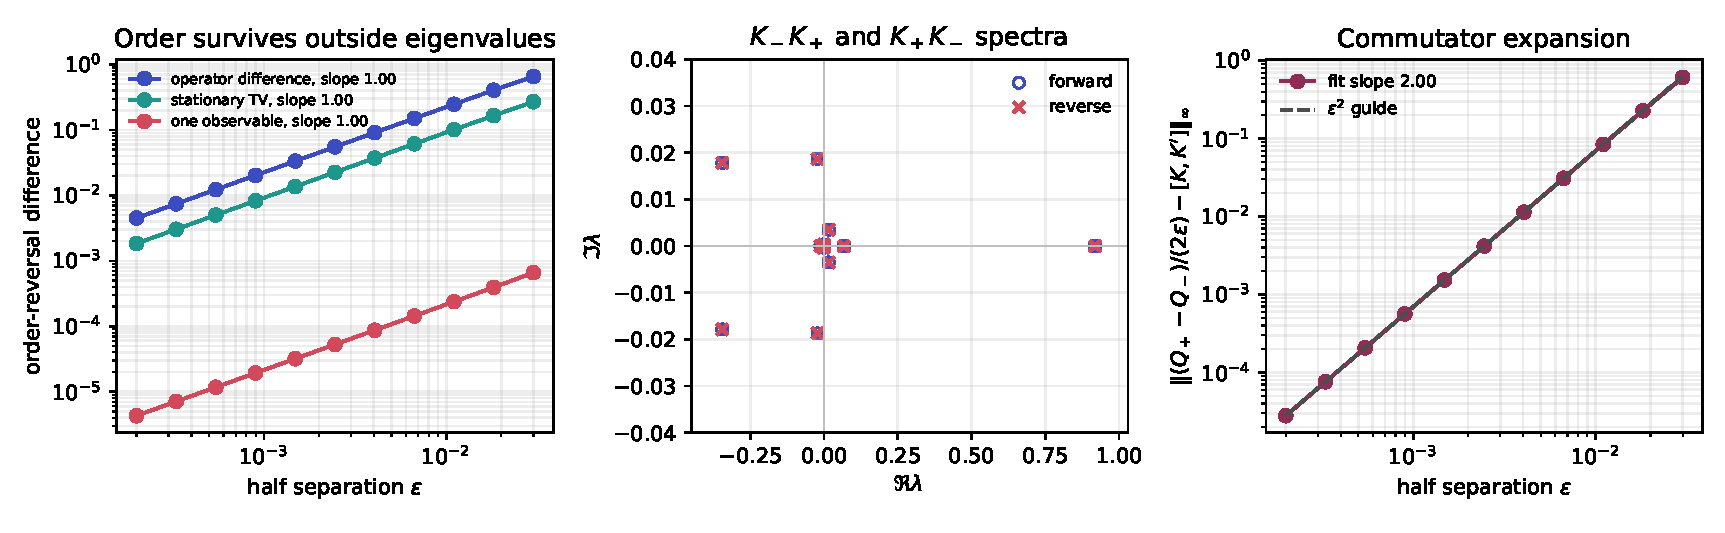
\includegraphics[width=\textwidth]{figures/two_step_blindness.pdf}
\caption{Two-step spectral blindness and operator order response.  Left:
matrix, stationary-law, and observable differences are first order in the
half separation.  Middle: forward and reverse non-Perron spectra at
$\varepsilon=0.02$ coincide visually and to the quantitative tolerance in the
text.  Right: after subtracting $[K,K']$, the normalized operator remainder is
quadratic.}
\label{fig:pair}
\end{figure}

\subsection{Orientation curvatures and the cubic law}

At $\sigma=0.05$, extrapolation through full dimension $2048$ gives
\begin{equation}\label{eq:numerical-curvatures}
 \chi_{\cK}(\uc)=-1.591713748,
 \qquad
 \chi_{\cQ}(\uc)=20.958960007.
\end{equation}
Their resolution-error slopes are $-1.99714$ and $-2.00115$.  Thus neither
minimal directed invariant vanishes at the tested parameter.  The parameter
atlas in \cref{fig:curvature} shows that signs and magnitudes vary strongly
with $u$ and $\sigma$; the curvatures are dynamical quantities, not universal
constants.

For symmetric triples, the relative errors in
\eqref{eq:symmetric-curvature} have fitted powers $2.00013$ for $\cK$ and
$1.99933$ for $\cQ$, confirming both the cubic Vandermonde factor and the
quadratic quotient correction.

\begin{figure}[t]
\centering
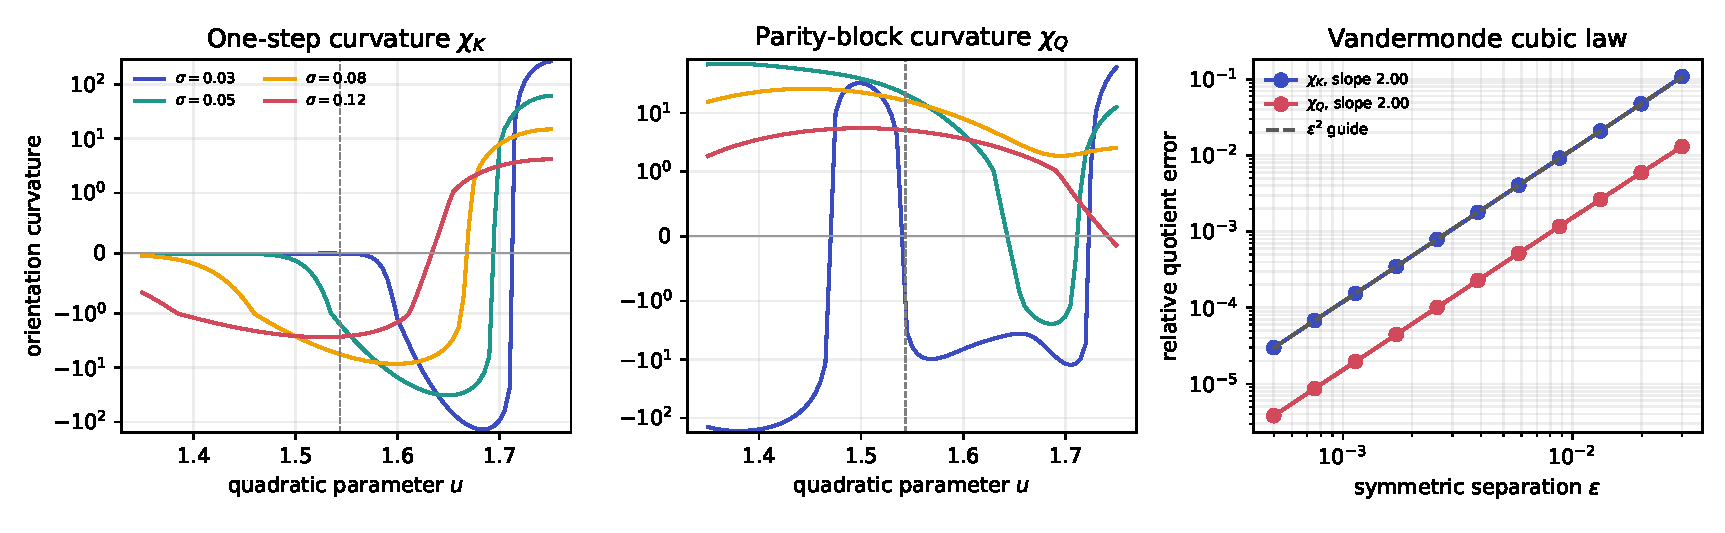
\includegraphics[width=\textwidth]{figures/orientation_curvature.pdf}
\caption{Orientation curvature.  Left and middle: one-step and frozen
parity-block curvature over $1.35\le u\le1.75$; the signed logarithmic axis is
linear between $-1$ and $1$.  The dashed line marks $\uc$.  Right: relative
error of the symmetric Vandermonde quotient, with the predicted
$\varepsilon^2$ law.}
\label{fig:curvature}
\end{figure}

\subsection{Resolution and logarithmic scales}

The left panel of \cref{fig:schedule} verifies the second-order continuum
limit.  For the macroscopic schedule experiment we set
\[
 p=2,\qquad \kappa=0.5,\qquad
 (\alpha,\beta,\gamma)=(1/4,1/2,1).
\]
At the finite schedule dimension $d=512$, the predicted limits of
$(\log T)^9\Omega_3$ and $(\log T)^9\Omega_6$ are $1.05249$ and $-13.96417$.
Direct traces through $\log T=20$ move toward those limits; the approach is
slow because the next expansion is only one inverse logarithm smaller.

The paired half increment and its Euler-transformed infinite tail satisfy
the constants from \cref{thm:pair-tail}: the normalized values approach
$-\kappa p/4=-0.25$ and $-\kappa/4=-0.125$.  This independently checks the
coefficient in the renormalized commutator tail.

\begin{figure}[t]
\centering
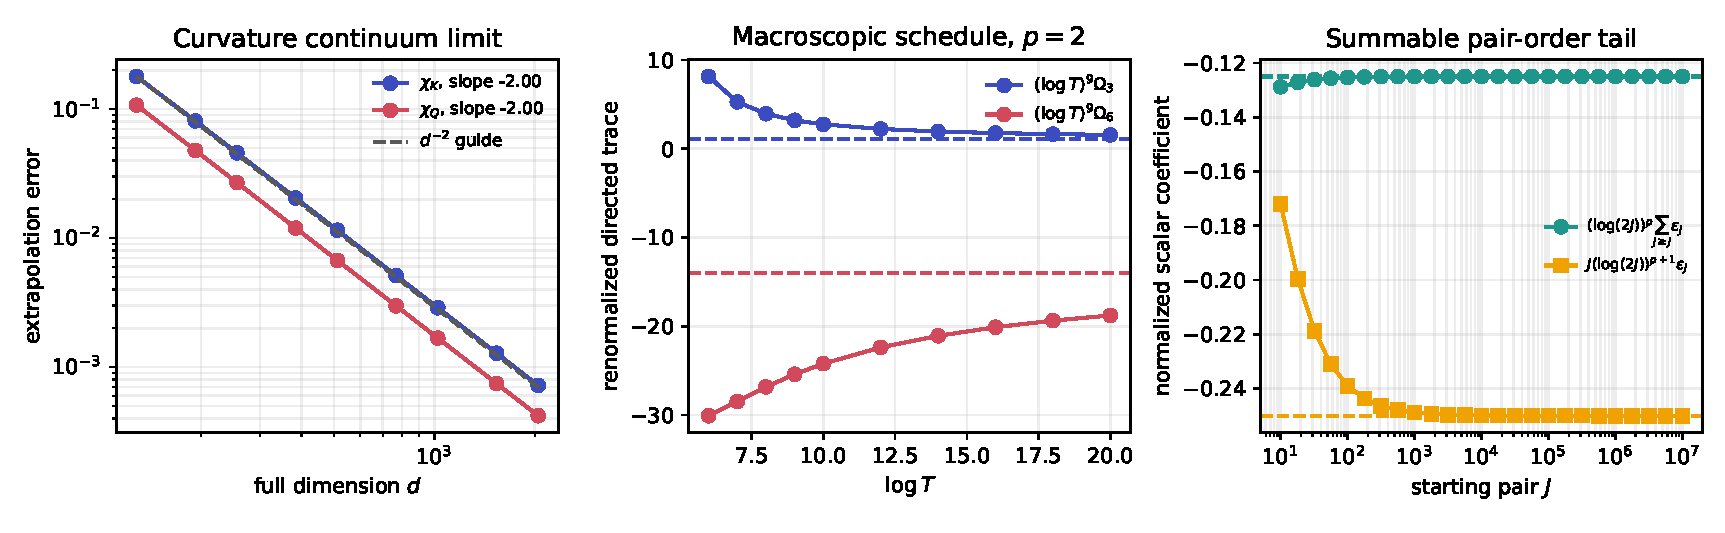
\includegraphics[width=\textwidth]{figures/resolution_schedule.pdf}
\caption{Continuum and schedule scaling.  Left: $d^{-2}$ convergence of both
orientation curvatures.  Middle: direct macroscopic traces for $p=2$ after
the $(\log T)^9$ renormalization; dashed lines are the finite-resolution
limits.  Right: normalized within-pair increment and infinite tail converging
to $-0.25$ and $-0.125$.}
\label{fig:schedule}
\end{figure}

\section{Consequences for the spectral program}
\label{sec:implications}

\subsection{The route that closes}

The most direct two-step proposal is now ruled out: reversing the order of
two frozen Gaussian kernels cannot change a nonzero eigenvalue, its algebraic
multiplicity, or any coefficient of the Fredholm determinant.  Therefore a
numerical difference between two such spectra is discretization, branch
matching, or roundoff---not a continuum arrow of time.

This is a structural statement, not a failure of the preceding continuum
spectrum.  The frozen resonances and cycle determinant remain valid.  What
fails is the additional interpretation that one two-step spectral list can
recover the orientation inside its pair.

\subsection{The route that remains}

Order survives in three increasingly demanding objects:
\begin{enumerate}[label=(\roman*),leftmargin=2.2em]
 \item the commutator $[\cK,\cK']$, observed through states, stationary laws,
 or inserted cocycle responses;
 \item the three-factor directed determinant, whose first distinguishing
 coefficient is $\Omega_3$; and
 \item the parity-compatible six-step determinant generated by three
 two-step blocks.
\end{enumerate}
The commutator tail is the largest of these for a logarithmic drive, but it is
traceless and state dependent.  Turning it into a universal scalar requires a
controlled cocycle, an observable, or an additional block.  The bare scalar
orientation is target independent but starts at $(\log T)^{-3p-3}$.

For a possible Hilbert--P\'olya route, this paper therefore replaces a vague
``time-ordered spectrum'' with falsifiable requirements.  A later object must
retain at least three-factor order, survive the relevant continuum and
small-noise limits, and eventually acquire a self-adjoint or scattering
interpretation with a correct counting law and arithmetic trace side.  None
of those later properties follows from the nonzero curvatures in
\eqref{eq:numerical-curvatures}.  In particular, no Riemann-zero conclusion is
drawn.

\section{Conclusion}

Two-step Gaussian quadratic products remember order in their action but not
in their nonzero spectrum.  The exact $AB$--$BA$ identity makes every
two-step eigenvalue and determinant reversal blind.  At the same time, a
first-order commutator changes stationary measures and weak observables, and
its accumulated logarithmic pair tail has an explicit nonzero renormalized
limit.

The first scalar orientation invariant requires three parameter values.  Its
Vandermonde factorization produces the intrinsic curvature
$\frac12\tr(\cA[\cA',\cA''])$.  Applied to $\cK_u^2$, it yields a minimal
parity-compatible six-step trace.  Macroscopic logarithmic orientation is
cubic in parameter differences, while consecutive orientation is summable.

These results are a useful negative gate and a constructive replacement.  A
route through raw paired eigenphases closes; a route through commutator
insertions and directed determinants remains mathematically defined.  Whether
that route survives small noise or admits a self-adjoint arithmetic lift is a
separate question.

\section*{Data and code availability}

The manuscript source, tests, machine-readable results, and figure scripts are
available at
\url{https://github.com/maris205/prime_dynamics_theory/tree/main/papers/RH-8-time-ordered-cycle-curvature}.
Exact reproduction commands are listed in the accompanying README.

\section*{Acknowledgments}

The author acknowledges the use of an AI language model for assistance with
mathematical cross-checking, code auditing, manuscript organization, and
typesetting.  The author verified the final arguments and assumes
responsibility for the content.

{\small
\bibliographystyle{plainnat}
\bibliography{references}
}

\end{document}
